\documentclass[a4paper,11pt]{report}
\usepackage[T1]{fontenc}
\usepackage[italian]{babel}
\usepackage{times}
\usepackage{graphicx}
\usepackage{algpseudocode}
\usepackage{algorithm}
\usepackage{algorithmicx}

\title{\Huge RELAZIONE ETHEREUM}
\author{Andrea Bedei}
\date{1 Aprile 2023}

\setcounter{tocdepth}{4}
\begin{document}
\maketitle
\tableofcontents
\listoffigures

\begin{abstract}% Abstract
In questa relazione si andrà a parlare del mondo delle blockchain e delle criptovalute, nella prima parte vengono descritte le caratteristiche principali e gli elementi base, alcuni anche visti a lezione. Poi si approfondiscono per quanto riguarda specificatamente il mondo Etherium, con algoritmi di criptaggio, specifiche dettagliate della rete. In aggiunta nel documento vengono descritte entrambe le strategie di convalida delle transazioni nonostante nel settembre 2022 la mainnet di Ethereum si è fusa con la Beacon Chain, completando la transizione della blockchain dalla proof of work alla proof of stake.
\end{abstract}

\chapter{Introduzione}
La criptovaluta è una nuova forma di denaro digitale alimentata dalla crittografia. Tutto è iniziato con Bitcoin, il quale permise di inviare fondi ovunque nel mondo senza l'uso di intermediari, cioè evitando che la nostra operazione passasse sotto un'autorità centrale come una banca o un governo, in modo tale che nessuno potesse sorvegliare, censurare o annullare le transazioni e soprattutto al fine di non condividere i nostri dati personali con terze parti.
Infatti, le transazioni di criptovalute collegano direttamente mittente e destinatario, nessun altro può avere accesso ai fondi altrui e nessuno può dire quali servizi una persona può o meno utilizzare. Tutto questo grazie alla tecnologia blockchain su cui operano le criptovalute.\\
La Blockchain è recentemente diventata una tendenza di ricerca, con grandi potenziali applicazioni in diversi settori e contesti. Una particolare tecnologia della Blockchain è lo smart contract, che è ampiamente utilizzato in contesti commerciali, come ad esempio in transazioni finanziarie di alto valore. Questo tuttavia ha implicazioni importanti per la sicurezza, infatti richiede: identificazione, autenticazione e cifratura dei dati. Tra questi, Ethereum è il più attivo. Quindi, esaminiamo le ricerche esistenti sulla sicurezza della rete di Ethereum, partendo dai primi anni della suo nascita fino ad arrivare alle ultime novità in fatto di ricerca. Si parlerà dei problemi di sicurezza, delle vulnerabilità nel programma e della crittografia che c'è dietro.

\section{Il contesto}
La prima parte di ricerca sulle criptovalute si svolge dopo il 2000, esse infatti erano interessanti per i ricercatori al fine di eseguire transazioni anonime.
La prima criptovaluta che nacque basata su Blockchain fu Bitcoin, proposto alla fine degli anni 2000, fino ad arrivare ai giorni nostri dove possiamo contare tantissime altre monete virtuali. 
Ad esempio, ad oggi ci sono circa 20.931 criptovalute monitorate da CoinMarketCap. Proprio grazie a Bitcoin il mercato ha potuto riconoscere il potenziale che offre la Blockchain, come la possibilità di avere un servizio decentralizzato, non manomettibile, trasparente e tracciabile.\\
Oltre a Bitcoin, un'altra applicazione Blockchain di grande successo è Ethereum, che utilizza un linguaggio di programmazione turing-completo per consentire agli utenti di sviluppare smart contract.\\
In questi anni si parla anche di un nuovo periodo digitale, definito come l'era della Blockchain 2.0, in cui diverse applicazioni possono essere costruite sulla base di smart contract. Alcuni esempi possono essere:
\begin{itemize}
\item Internet of Things
\item Assistenza sanitaria
\item Servizi commerciali
\item Scambio sicuro di dati
\end{itemize}

\chapter{Blockchain}

\section{Definizione}
La blockchain può essere definita come un registro digitale distribuito, in grado di memorizzare record di dati, chiamati \textbf{transazioni} in modo sicuro, verificabile e permanente. \\
\begin{figure}[htbp] 
\begin{center}
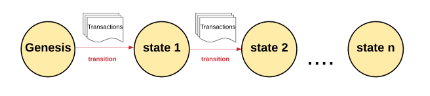
\includegraphics[width=8cm]{img/genesis.png} 
\end{center}
\caption{Rappresentazione degli stati della blockchain \cite{genesis}}
\end{figure}
\\Dopo aver scritto i dati in un blocco non possono essere modificati senza che vengano alterati tutti i blocchi successivi, questo per la natura del protocollo e dello schema di validazione, infatti l'unico modo per farlo necessiterebbe del consenso della maggioranza della rete. La blockchain è quindi rappresentabile come una grande catena di blocchi collegati tra loro e resi sicuri attraverso la crittografia. In ogni blocco possono essere presenti una o più transazioni e contiene un puntatore hash al blocco precedente e una marca temporale. \\

\begin{figure}[htbp] 
\begin{center}
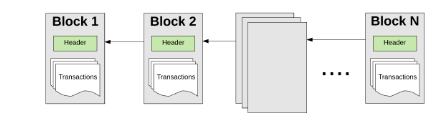
\includegraphics[width=8cm]{img/blkc.png} 
\end{center}
\caption{Rappresentazione dei blocchi della blockchain. \cite{genesis}}
\end{figure}

\newpage
La natura cooperativa rende robusto e sicuro il processo di validazione ma questo porta tempi di aggiornamento non trascurabili, a causa del processo di validazione dei blocchi e alla sincronizzazione di tutta la rete. L'utilizzo di questa tecnologia permette di superare il problema dell'infinita riproducibilità di un bene digitale e della doppia spesa, ed essa permette di fare a meno di un server centrale o di un'autorità.\\
Quindi in altre parole possiamo definire la Blockchain come un sistema distribuito, in cui tutti i nodi sono indipendenti nell'eseguire azioni, ma nel frattempo strettamente uniti nel mantenimento di un libro mastro identico.\\
Inoltre, ogni transazione dopo essere stata verificata verrà inserita nell'ultimo blocco, il quale verrà collegato all'ultimo pezzo della catena impostando l'hash del blocco precedente come input nel calcolo dell'hash del blocco corrente. Solo quando la maggior parte dei miner raggiunge il consenso questa transazione può essere registrata nel libro mastro della Blockchain.\\ 
\newpage
\section{Tipologie}

La Blockchain può essere classificata in due categorie principali: \textbf{permissionless} e \textbf{permissioned}. Nel primo caso, tutti possono unirsi o uscire arbitrariamente, mentre la seconda aggiunge delle regole di gestione dei membri per porre restrizioni ai partecipanti, in questo modo solo i membri selezionati hanno i diritti di accesso e mantenimento del libro mastro. \\
In generale, la Blockchain pubblica è più popolare grazie alla sua quasi completa conformità agli obiettivi di progettazione originali.
A livello di Blockchain, bisogna garantire che la tecnologia di registro distribuito sia corretta e coerente tra tutti i nodi. Pertanto, abbiamo bisogno di avere un meccanismo di consenso. Esso dovrebbe considerare la presenza di utenti malintenzionati, che cercano di massimizzare i loro benefici anche a costo di distruggere l'intero sistema. I meccanismi di consenso esistenti possono essere classificati in deterministici e non deterministici. Nella prima categoria, una volta aggiunto il blocco alla catena principale tutte le transazioni nel blocco vengono convalidate e non possono più essere modificate. Invece, i tipici meccanismi di consenso non deterministico sono nominati \textbf{Proof of Work} e \textbf{Proof of Stake}. In questo tipo di consenso, anche se il blocco viene convalidato e aggiunto alla catena principale, può essere invalidato in seguito. Poiché ci sono dei fork, cioè due blocchi figli validi appartenenti allo stesso blocco padre che possono anche essere estratti contemporaneamente, uno di essi verrà scartato se la catena in cui si trova l'altro blocco diventa la catena più lunga.

\begin{figure}[htbp] 
\begin{center}
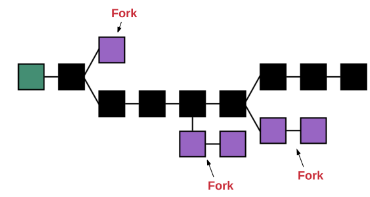
\includegraphics[width=8cm]{img/fork.png} 
\end{center}
\caption{Esempio di fork. \cite{genesis}}
\end{figure}

\chapter{Smart contract}
\section{Definizione}
Uno smart contract può essere definito come un protocollo di transazione o un programma che ha lo scopo di controllare, eseguire o documentare automaticamente eventi legalmente rilevanti secondo i termini di un contratto o di un accordo. Gli obiettivi di essi sono rimuovere intermediari, abbattere i costi ed evitare le perdite per frode. Gli smart contract sono spesso associati alle criptoavalute e quelli introdotti da Ethereum sono le basi per le applicazioni di finanza decentraliazzata(DeFi).\\
L'esempio più antico di tecnologia equivalente all'implementazione di smart contract sono proprio i distributori automatici. Questi infatti a input specifici garantiscono degli output predeterminati. Il distributore eroga la merce solo se sono soddisfatti tutti i requisiti e se ne manca solo uno l'operazione non si compirà.\\
Ethereum propone una versione più forte del concetto di smart contract rispetto a quella di Bitcoin, basata sul linguaggio Solidity, che è turing completo. Infatti, a partire da Bitcoin sempre più criptovalute supportano linguaggi di tipo scripting che consentono smart contract più avanzati tra parti non affidabili.\\
Durante il  corso del tempo la definizione di contratto intelligente è variata. Il NIST (National Institute of Standards and Technology) lo definisce come una raccolta di codice e dati che viene distribuito attraverso transazioni firmate crittograficamente sulla rete blockchain, quindi non è necessariamente correlato al concetto classico di contratto, ma può essere un qualsiasi tipo programma eseguibile. Uno smart contract può essere anche comparato a una stored procedure, questo perchè gli eventi tra le parti avvengono rigorosamente e non possono essere manipolati dopo che una transazione con dettagli specifici del contratto è stata archiviata in una blockchain o in un registro distribuito. Questo perchè l'effettiva esecuzione dei contratti è controllata e verificata dalla piattaforma e non da programmi arbitrari.
\begin{figure}[htbp] 
\begin{center}
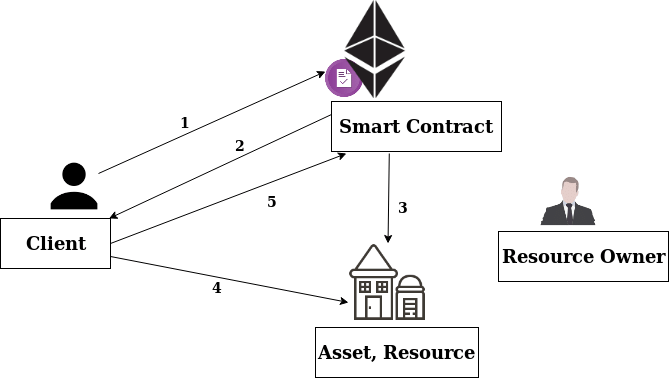
\includegraphics[width=8cm]{img/smrt.png} 
\end{center}
\caption{Vista generica sul concetto di smart contract.\cite{smartContract}}
\end{figure}


\section{Caratteristiche degli smart contract}
Proposti per la prima volta da Szabo, gli smart contract hanno generalmente le seguenti caratteristiche:
\begin{enumerate}
\item \textbf{Auto-esecuzione:} sono innescati direttamente dalle transazioni, senza la necessità di interazione manuale.
\item \textbf{Auto-applicazione:} una volta attivati, non è possibile impedirne l'esecuzione.
\item \textbf{Trasparenza:} gli smart contract sono noti a ciascun nodo della rete Blockchain, poiché la loro correttezza deve essere verificata dalla maggior parte dei nodi.
\item \textbf{Flessibilità:} possono adattarsi alle diverse esigenze dello scenario.
\item \textbf{Sicurezza:} devono essere sicuri.
\end{enumerate}
La sicurezza degli smart contract è importante perchè tali contratti sono generalmente utilizzati in contesti finanziari e quindi sono un obiettivo attraente per i criminali informatici motivati finanziariamente e criminalmente.\\
Inoltre, qualsiasi violazione possibile può avere un impatto sulla fiducia degli utenti e quindi sull'utilizzo dello smart contract.\\
Ci sono state alcune violazioni negli ultimi anni, come ad esempio attraverso l'hackeraggio del Decentralized Autonomous Organization\footnote{Organizzazioni basate su blockchain che sono di proprietà collettiva e gestite dai loro stessi membri, utenti e team.} (DAO) o di Parity\footnote{Parity Ethereum è una soluzione software open source che consente a un individuo di eseguire un nodo sulla rete pubblica Ethereum o su qualsiasi altra rete blockchain che utilizza il protocollo Ethereum. Esso permette anche di sostituire il meccanismo di consenso utilizzato.}. Più recentemente, nel 2018, è stato hackerato un gioco denominato Dapp, in cui la tecnica usata è denominata front-running e consiste nell'inserire record di transazioni nella rete Blockchain con commissioni elevate per impedire che altre transazioni vengano eseguite, rubando circa 10000 ETH.

\section{Funzionamento}
La distribuzione di uno smart contract su una blockchain avviene attraverso una transazione da un portafoglio alla blockchain. L'operazione comprende il codice compilato dello smart contract e un indirizzo speciale del destinatario. Tale transazione deve essere quindi inclusa in un blocco, che verrà poi aggiunto alla blockchain, nel quale il codice verrà eseguito per stabilire lo stato iniziale dello smart contract. Una volta che uno smart contract viene distribuito, non può più essere aggiornato. I clienti finali interagiscono con uno smart contract attraverso le transazioni. Tali transazioni potrebbero comportare la modifica dello stato e l'invio di criptovalute da uno smart contract ad un altro o anche più semplicemente fra due conti.

\section{Ethereum}
La più popolare blockchain per l'esecuzione di smart contract è Ethereum. Su di essa, gli smart contract sono tipicamente scritti in un linguaggio di programmazione turing-completo chiamato Solidity e compilati in bytecode a basso livello per essere eseguiti dalla Ethereum Virtual Machine.\\
I processi su una blockchain sono deterministici, in modo da garantire la tolleranza ai guasti. Tuttavia, l'applicazione degli smart contract nel mondo reale richiede della casualità, ad esempio come nei giochi dei casinò. Infatti, la tecnologia blockchain riduce i costi per lo svolgimento di questi giochi. La casualità sulla blockchain può essere implementata utilizzando block hash oppure degli smart contract speciali, un esempio è RANDAO.

\section{Registro pubblico e privacy per Ethereum}
Visto che gli smart contract di Ethereum si basano su una blockchain pubblica chiunque può monitorare in qualsiasi momento i trasferimenti di risorse. Un esempio è il fatto che chiunque può in ogni momento controllare se qualcuno ha inviato del denaro al suo indirizzo. Tutto questo però non influisce sulla privacy, questo perché Ethereum è una rete pseudonima, cioè le transazioni sono pubblicamente legate a un indirizzo crittografico univoco e non all'identità della persona. In questo modo possiamo proteggere la privacy delle persone dagli osservatori.

\section{Problemi di sicurezza}
Uno smart contract basato su blockchain è visibile a tutti gli utenti della blockchain stessa. Tuttavia, questo crea una situazione in cui i bug sono visibili a tutti e questo può portare attacchi da parte di persone malevole.

\section{Conclusioni e casi d'uso}
In parole semplici, gli smart contract sono dei programmi informatici risiedenti sulla blockchain che possono fare qualsiasi cosa, eseguire calcoli, creare valuta, memorizzare dati, creare NFT o persino generare immagini.

\chapter{Ethereum}
\section{Definizione di Ethereum}
Ethreum può essere definito come una blockchain decentralizzata del Web 3.0 open source per la creazione e la pubblicazione peer to peer di smart contract, ossia contratti intelligenti.\\
Per il momento si trova al secondo posto per la sua capitalizzazione di mercato.

\section{Come nasce Ethereum?}
Ethereum è stato creato nel 2013 dal programmatore Vitalik Buterin. Nel 2014 il lavoro di sviluppo è iniziato e la rete è diventata operativa.
Ethereum fu lanciato nel 2015 e si basa sull'innovazione di Bitcoin, ma con alcune grandi differenze: entrambi consentono di utilizzare il denaro digitale senza intermediari, ma Ethereum è programmabile, quindi le persone hanno la possibilità anche di creare e distribuire applicazioni decentralizzate sulla sua rete. 


\section{Cosa può fare?}
Chiunque può creare app che utilizzino la blockchain per archiviare dati oppure per altri tipi di attività. Ciò si traduce in una blockchain generica che può essere programmata per qualsiasi compito. Quindi, a differenza di Bitcoin che è solo una rete di pagamento, Ethereum dà un infinità di possibilità, tra cui: 
\begin{itemize} % elenco puntato
\item \textbf{Attività bancarie:} per avere l'accesso a un servizio finanziario si necessita solo di una connessione ad internet. 
\item \textbf{Internet privato:} non c'è la necessità di fornire informazioni personali per usare le funzionalità di un app Ethereum.
\item \textbf{Rete peer-to-peer:} vengono stretti accordi solo tra un ricevente e un destinatario senza intermediari.
\item \textbf{Anti Censura:} nessuno ha il controllo su Ethereum.
\item \textbf{Garanzie:} le persone hanno la garanzia che i fondi verranno trasferiti.
\item \textbf{Tutti gli sviluppi sono compatibili:} visto che le app sono costruite sulla stessa blockchain con uno stato globale condiviso, possono essere assemblate a vicenda e questo permette di creare prodotti ed esperienze migliori in ogni momento. 
\end{itemize}

\section{Tipi di account}
Ethereum adotta una modalità di account simile al meccanismo di gestione dell'account nel sistema bancario convenzionale. Esistono due tipi di account: di \textbf{proprietà esterna}, con la sigla EOA e \textbf{a contratto}. Entrambi i tipi di account sono identificati in modo univoco da un indirizzo di 20 byte, che è proprio la loro identità nella rete Ethereum. Gli EOA sono controllati da coppie di chiavi pubbliche/private, utilizzate principalmente per gestire la moneta e per interagire con gli smart contract inviando transazioni. Invece gli account a contratto sono controllati da codici senza chiavi e utilizzati principalmente per implementare diversi requisiti di funzione e registrare le modifiche allo stato del contratto come le transazioni eseguite e la modifica del saldo.\\
A differenza degli EOA, gli account a contratto non possono inviare transazioni ma possono inviare chiamate tramite messaggi per chiamare altri contratti.\\
\begin{figure}[htbp] 
\begin{center}
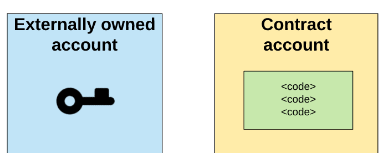
\includegraphics[width=7cm]{img/ac.png} 
\end{center}
\caption{Tipi di account. \cite{genesis}}
\end{figure}
\\Per quanto riguarda le similitudini, entrambi i tipi di account hanno uno \textbf{stato} in cui viene memorizzato: il nonce (numero di transazioni provenienti dall'indirizzo), il saldo delle risorse e l'hash del nodo radice dell'albero, l'hash del nodo corrente e tutti gli stati memorizzati. \\
\begin{figure}[htbp] 
\begin{center}
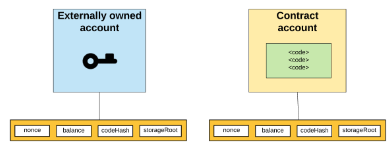
\includegraphics[width=9cm]{img/ndi.png} 
\end{center}
\caption{Contenuto informativo dell'account. \cite{genesis}}
\end{figure}

\section{Stato a livello mondiale}
Lo stato globale di ethereum consiste in una mappatura tra gli stati e gli indirizzi degli account. Tale mappatura è memorizzata in una struttura ad albero denominata albero di Merkle Patricia.\\
Esso è  è un albero in cui ogni foglia (nodo) è etichettato con l'hash crittografico di un blocco di dati e ogni nodo che non è una foglia (chiamato ramo) è etichettato con l'hash crittografico delle etichette dei suoi nodi figli. Un tale albero consente una verifica efficiente e sicura del contenuto di una struttura dati di grandi dimensioni. Un albero hash è una generalizzazione di un elenco hash e di una catena hash.
Per dimostrare che un nodo foglia fa parte di un determinato albero hash binario è necessario calcolare un numero di hash proporzionale al logaritmo del numero di nodi foglia nell'albero. Al contrario, in un elenco di hash, il numero è proporzionale al numero di nodi foglia. Un albero Merkle Patricia è quindi un esempio efficiente di uno schema crittografico.

\begin{figure}[htbp] 
\begin{center}
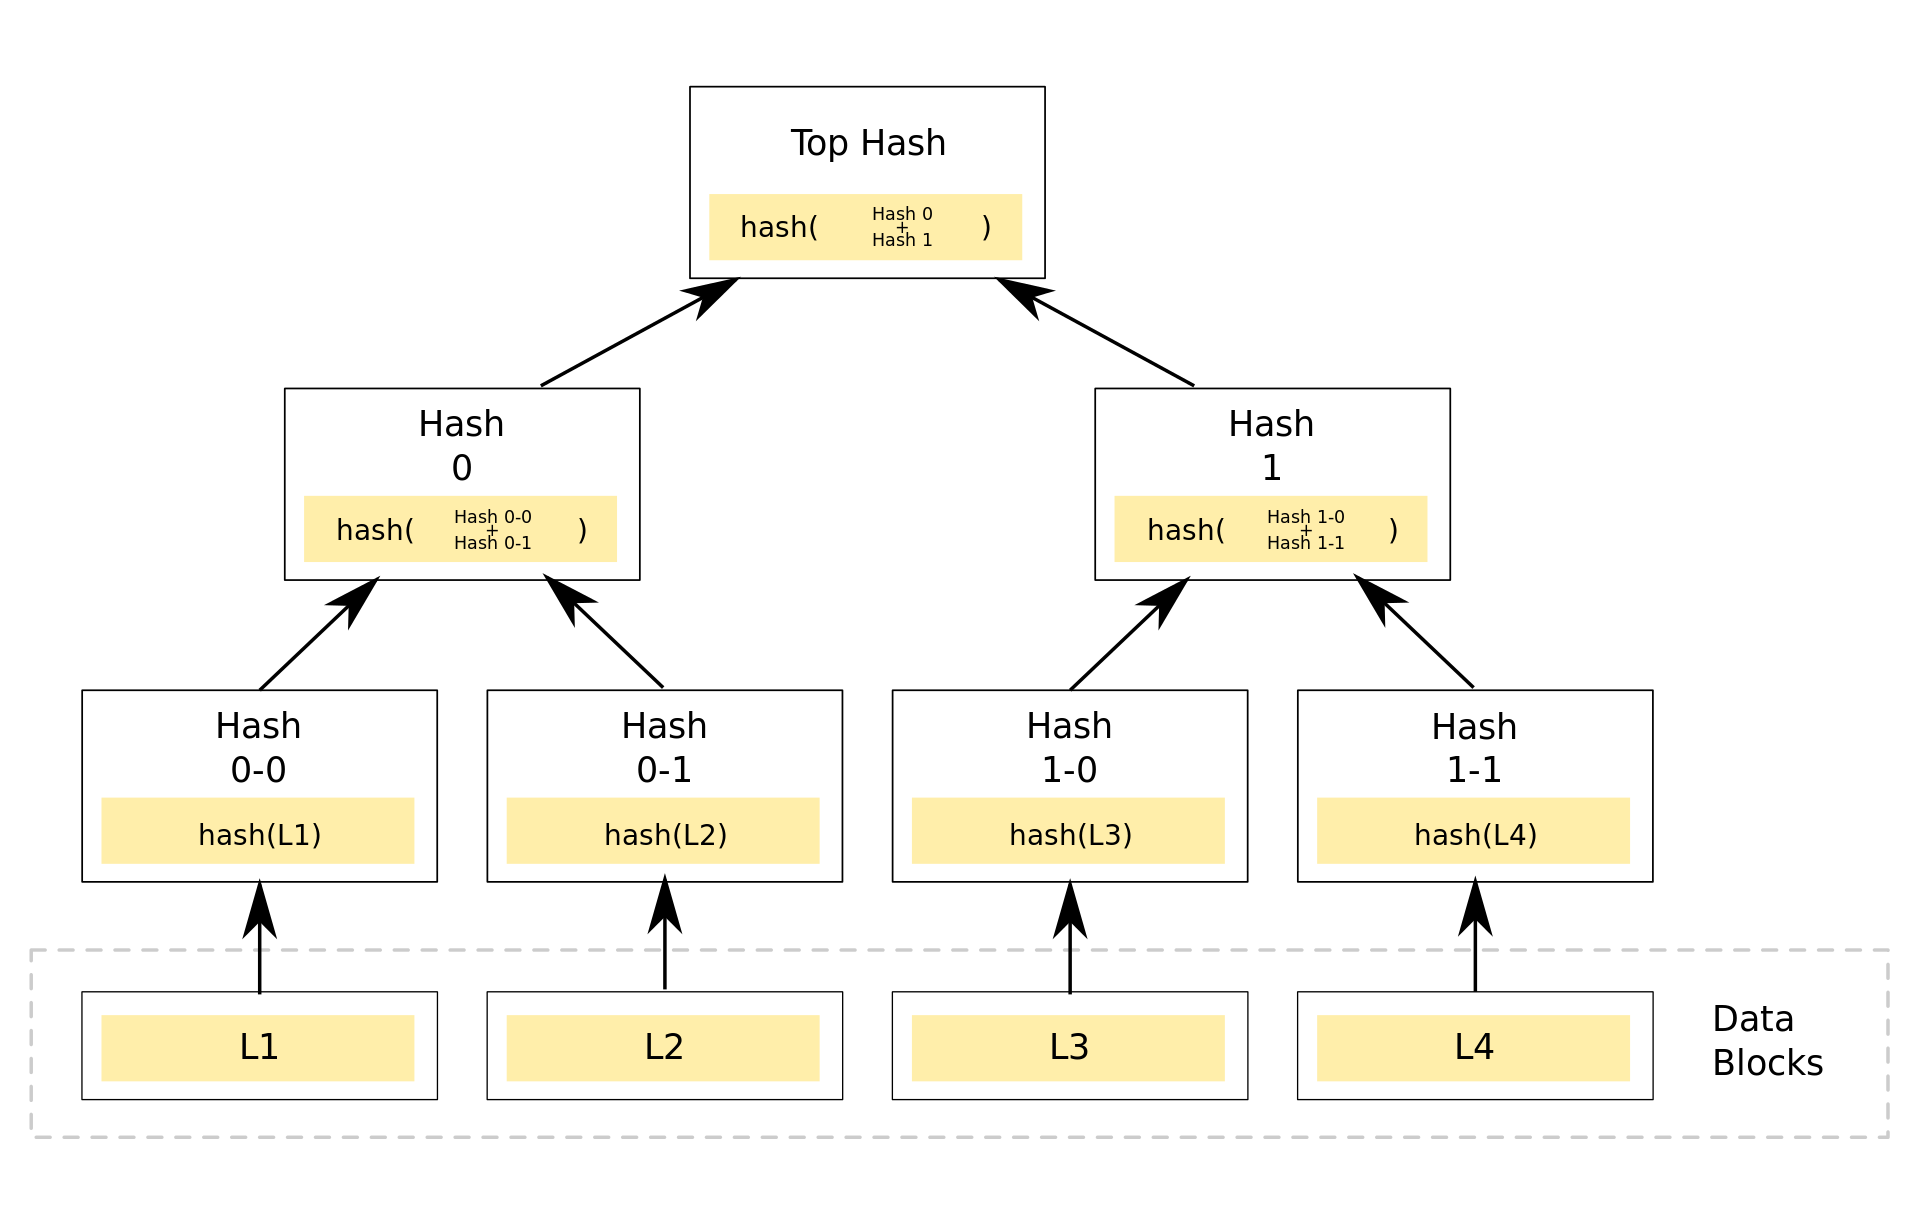
\includegraphics[width=9.5cm]{img/hs.png} 
\end{center}
\caption{Albero di Merkle Patricia. \cite{albero}}
\end{figure}
\newpage
I dati della parte inferiore vengono generati suddividendo in porzioni i dati che vogliamo archiviare, quindi prendendo l'hash di ciascuna sezione e ripeteremo il processo fino a quando il numero totale di hash rimanenti diventa uno solo, cioè l'hash radice.\\
Le caratteristiche di questi tipi di alberi:
\begin{itemize}
\item Molti nodi foglia nella parte inferiore che contengono i dati.
\item Insieme di nodi intermedi, dove l'hash di ciascuno è la combinazione dell'hash dei due nodi figli.
\item Un singolo nodo radice, anch'esso con l'hash calcolato dai due nodi figli.
\end{itemize}

\section{I blocchi}
I blocchi sono un insieme di transazioni, in cui è anche presente un hash del blocco precedente della catena per collegare i blocchi tra di loro. In aggiunta l'hash del blocco corrente viene calcolato crittograficamente dai dati del blocco stesso: questo impedisce che possano verificarsi delle frodi, infatti un minimo cambiamento nella cronologia invaliderebbe tutti i blocchi successivi e tutti quelli che eseguono la blockchain se ne accorgerebbero.
Affinché tutti i blocchi della rete siano sincronizzati, le transazioni vengono raggruppate a blocchi, cioè tantissime transazioni vengono prima inviate, poi approvate e sincronizzate in una sola volta.\\
\begin{figure}[htbp] 
\begin{center}
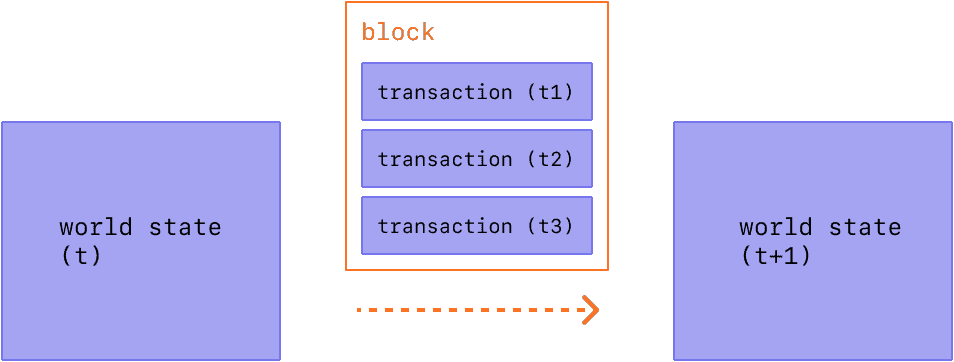
\includegraphics[width=9cm]{img/tx-block.png} 
\end{center}
\caption{Struttura del blocco. \cite{ether}}
\end{figure}
\\Quindi i blocchi sono ordinati in modo rigoroso, così come anche le transazioni all'interno del singolo blocco.

\newpage

\section{Mining}
\begin{figure}[htbp] 
\begin{center}
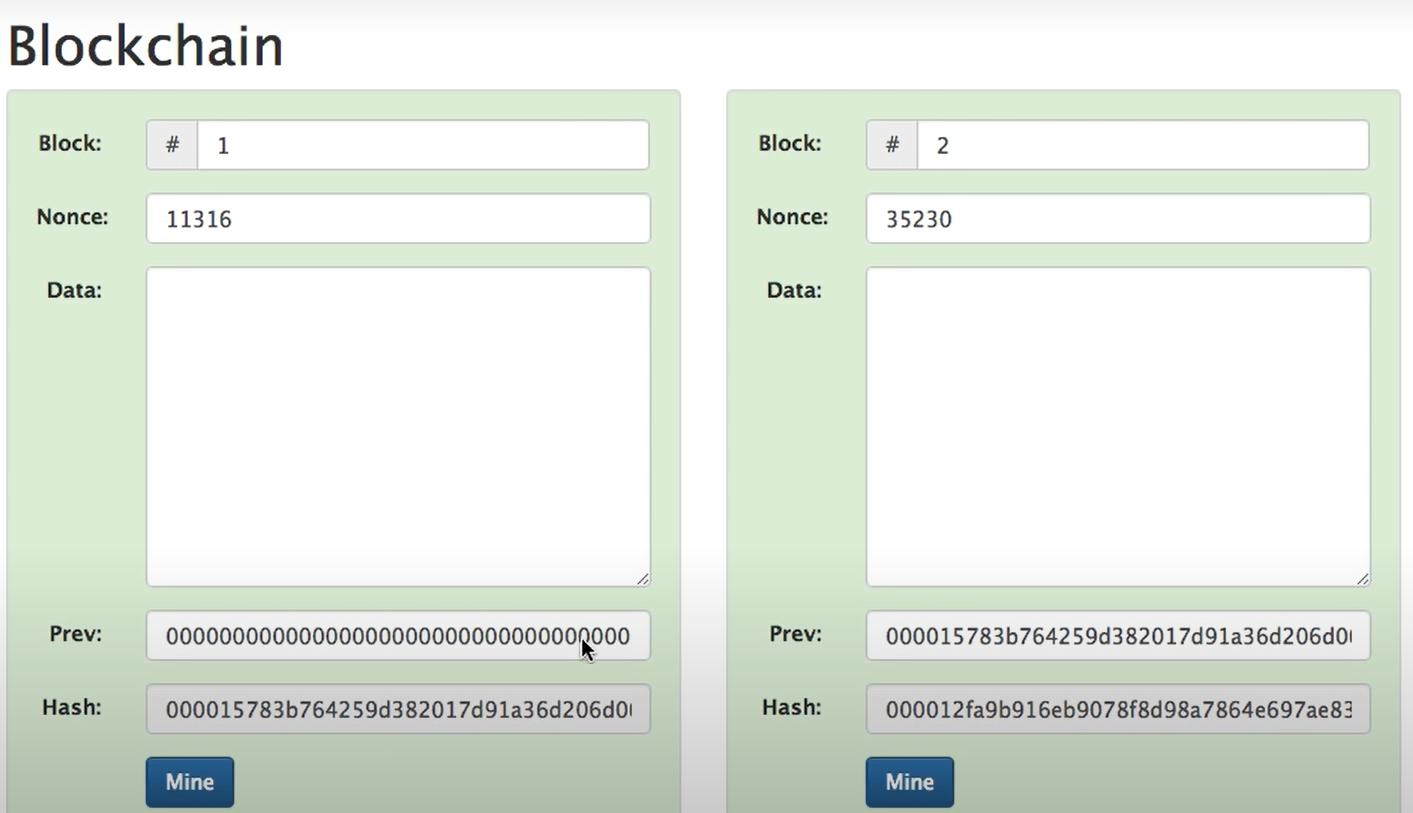
\includegraphics[width=9cm]{img/mm.png} 
\end{center}
\caption{Primi due blocchi di una blockchain. \cite{mine}}
\end{figure} 
Tutti i partecipanti delle rete cooperano per raggruppare le nuove transazioni del nuovo blocco e dopo averlo realizzato (Mining), il nuovo blocco viene propagato al resto della rete. Il nodo viene infatti inserito in fondo alla catena e il processo di mining continua. Tale processo, definito anche processo di consenso, viene illustrato nel protocollo di Ethereum denominato Proof of work.\\
I nodi attivi di mining usano una quantità variabile di tempo, di energia, ma sopratutto di potenza di calcolo per produrre un cosiddetto certificato di legittimità per il blocco che propagano sulla rete. Questo processo aiuta a proteggere il sistema da attacchi spam e DoS, anche perchè questi certificati sono costosi da produrre.\\
Gli altri miner (coloro che non hanno convalidato il blocco) ricevono un messaggio della presenza di un nuovo blocco con il relativo certificato di legittimità valido e devono accettarlo come blocco successivo della blockchain.\\
La quantità esatta di tempo richiesta da ogni miner per la creazione del certificato varia casualmente con elevata frequenza. Questo rende impossibile che due miner convalidino contemporaneamente un blocco successivo proposto e ciò fa sì che il blocco venga accettato come blocco successivo senza conflitti. Comunque, anche se accedesse che due blocchi vengano convalidati nello stesso istante, esiste un protocollo di risoluzione.

\subsection{Contenuto di un blocco}
\begin{figure}[htbp] 
\begin{center}
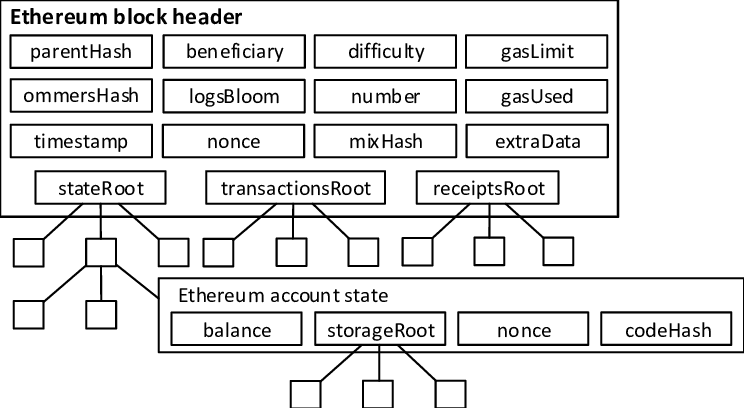
\includegraphics[scale=0.45]{img/block.png}
\end{center}
\caption{Elementi del blocco. \cite{block}}
\end{figure} 

Al suo interno un blocco contiene:
\begin{itemize} % elenco puntato
\item \textbf{Timestamp:} orario in cui il blocco è stato minato.
\item \textbf{BlockNumber:} numero del blocco, che corrisponde alla lunghezza della blockchain.
\item \textbf{BaseFeePerGas:} commissione minima in gas(piccola tassa pagata dagli utenti per compensare l'utilizzo di energia elttrica per l'elaborazione) affinché una transazione venga inclusa nel blocco.
\item \textbf{Difficulty:} quantità di lavoro necessaria per minare il blocco.
\item \textbf{MixHash:} identificatore unico per il blocco.
\item \textbf{ParentHash:} identificatore unico per il blocco precedente.
\item \textbf{Transactions:} le transazioni del blocco.
\item \textbf{Nonce:} un hash che, in combinazione con il mixHash, verifica se il blocco ha superato la Proof of Work.
\item \textbf{StateRoot:} intero stato del sistema (saldi degli account, codice del contratto e i nonce dell'account).
\end{itemize}

\subsubsection{Funzione aggiuntiva del Nonce}
Il nonce ha una funzionalità aggiuntiva: se si trasmette la stessa transazione più volte sperando che venga eseguita dai minatori molte volte, questi invece la identificheranno come una transazione ripetuta e quindi la scarteranno.

\subsection{Transazioni}
Le transazioni verranno trasmesse a ogni minatore per l'esecuzione e cambieranno lo stato di archiviazione della Blockchain dopo aver raggiunto il consenso. \\
Ogni transazione specificherà il suo nonce, il prezzo per le gas fee, il pagamento massimo delle gas fee per questa particolare transazione, il valore trasferito, il destinatario, i dati di input e la firma.

\subsubsection{Meccanismo delle Gas Fee} 
Il meccanismo di tariffazione delle gas fee svolge un ruolo chiave in molti aspetti: 
\begin{enumerate}
\item  Compensazione e incentivazione per i minatori che eseguono e memorizzano le transazioni.
\item  Contromisura per prevenire attacchi DoS, come utenti malintenzionati che inviano transazioni complesse di calcolo.
\end{enumerate}
Possiamo dire che ogni calcolo che viene eseguito a seguito di una transazione è soggetto a una commissione. Tale commissione viene denominata \textit{carburante}.
Il prezzo del carburante è la quantità di Ether che le persone sono disposte a spendere per ogni unità di esso. In ogni transazione il mittente imposta un limite di carburante e il suo prezzo. Il prodotto tra i due valori rappresenta l'imposto massimo da pagare per l'esecuzione della transazione. Tale somma verrà invita all'indirizzo del miner che ha approvato la transazione.
\begin{figure}[htbp] 
\begin{center}
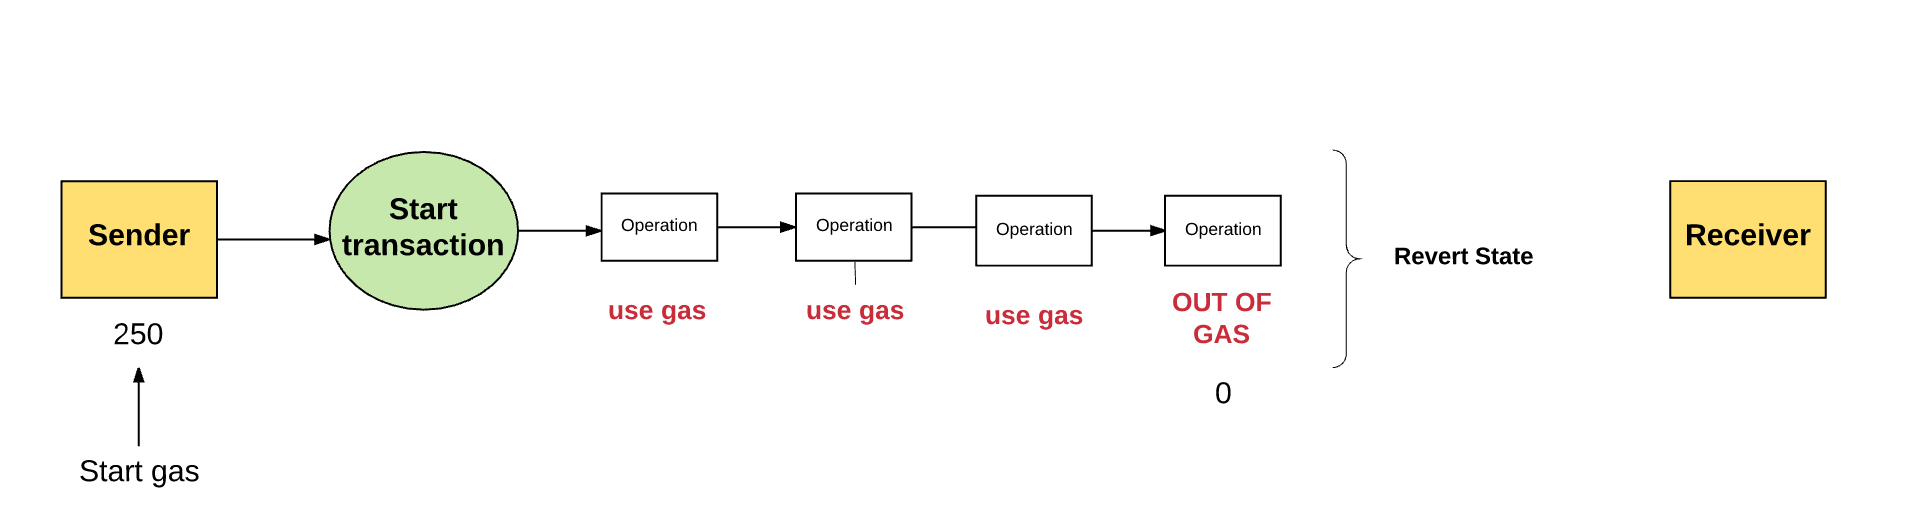
\includegraphics[width=9cm]{img/gas.png} 
\end{center}
\caption{Struttura del meccanismo delle commissioni. \cite{genesis}}
\end{figure}

\subsubsection{Tecnologia chiamata zk-SNARKs}
La tecnologia chiamata zk-SNARKs (Zero-Knowledge Succinct Non-Interactive Argument of Knowledge) è una forma di crittografia a zero conoscenza utilizzata per dimostrare la conoscenza di una determinata informazione senza doverla rivelare effettivamente.\\ In pratica, questo significa che con zk-SNARKs è possibile dimostrare di avere una determinata informazione, come ad esempio una password, senza rivelare la password stessa o qualsiasi altra informazione associata. Ciò è reso possibile utilizzando una combinazione di tecniche di crittografia avanzate, come la crittografia asimmetrica, la firma digitale e la crittografia a curva ellittica.\\
In Ethereum, gli zk-SNARKs vengono utilizzati per fornire un livello di privacy alle transazioni attraverso la funzionalità "private transactions". In questa funzionalità, gli zk-SNARKs vengono utilizzati per dimostrare la correttezza di una transazione senza rivelare alcuna informazione associata ad essa, come l'importo della transazione o il destinatario.\\ In pratica, una transazione privata in Ethereum utilizza uno smart contract di verifica della transazione. Questo contratto intelligente richiede una prova della correttezza della transazione sotto forma di una prova zk-SNARK. Essa viene creata dall'utente che effettua la transazione utilizzando i dati della relativa transazione, come l'importo e il destinatario, insieme a un insieme di parametri pubblici.\\ La creazione della prova zk-SNARK è un processo complesso che richiede una serie di passaggi matematici, tra cui la creazione di un circuito aritmetico, la generazione di chiavi pubbliche e private, e la creazione della prova stessa. Tuttavia, una volta che la prova zk-SNARK è stata creata, può essere utilizzata per dimostrare la correttezza della transazione senza rivelare alcuna informazione associata ad essa.\\
Quando la prova zk-SNARK viene presentata al contratto intelligente di verifica della transazione, il contratto esegue una verifica della prova per confermare che la transazione sia corretta. Se la prova è valida, il contratto intelligente attiva la transazione e la trasferisce sulla blockchain, senza rivelare alcuna informazione associata alla transazione.\\
In questo modo, gli zk-SNARKs offrono una forma di privacy per le transazioni su Ethereum, consentendo agli utenti di effettuare transazioni senza dover rivelare informazioni sensibili a terze parti.


\subsection{Tempo di blocco e dimensione}
Viene definito il tempo di blocco come il tempo per minare un elemento.
Il tempo medio per minare un blocco è tra i 12/14 secondi e viene rivalutato dopo ogni validazione di un elemento. Il tempo di blocco previsto è impostato come una costante a livello di protocollo ed è usata per proteggere la sicurezza della rete in caso in cui i miner aumentino la loro potenza di calcolo. Il tempo di blocco medio viene quindi confrontato con il tempo di blocco previsto e in base al risultato si sceglierà se aumentare o diminuire la difficoltà nell'intestazione dell'elemento.\\
La difficoltà del blocco influenza il nonce, infatti esso è un hash che viene calcolato quando si esegue il mining del blocco. La relazione matematica di difficoltà del blocco e il suo relativo nonce è:\\  \begin{center}
$n \leq \frac{2^{256}}{Diff}$
\end{center} dove Diff è la difficoltà.
La dimensione del blocco non si misura in numero di transazioni ma come somma di gas. Il gas in Ethereum è l'unità di misura utilizzata per misurare il lavoro svolto per effettuare transazioni o in generale interazioni nella rete.
Per ogni blocco il numero di gas deve andare da un minimo di 15 milioni a un massimo di 30 milioni.

\section{Dettagli sul mining}
Ora elenchiamo passo dopo passo come si svolge il mining delle transazioni Ethereum, descrivendo le operazioni dettagliatamente:
\begin{enumerate} % elenco numerato
\item Come primo passo l'utente firma una richiesta di transazione con la chiave privata del proprio account. Questo prova che la transazione sia stata creata dal mittente. Il processo di firma viene gestito da un client chiamato Geth. 
\item L'utente poi trasmette la richiesta della transazione all'intera rete.
\item Una volta ricevuta la richiesta, ogni nodo mette la richiesta nella propria mempool locale, la quale contiene un elenco di richieste di transazioni che non sono ancora state confermate e inserite in un blocco.
\item A questo punto un nodo di mining unisce queste richieste e crea un potenziale nodo e lo fa in modo da massimizzare le commissioni sulle transazioni.\\ Il compito del nodo di mining è quello di verificare ogni richiesta di transazione, alcuni esempi possono essere transazioni senza firma dell'utente oppure con formato scorretto della richiesta, dopodiché esegue il codice della richiesta, cambiando lo stato della propria copia locale dell'Ethereum Virtual Machine.\\
In questo momento inizia il processo di creazione del certificato di legittimità, Proof of Work.
\item A questo punto se tutto è andato a buon fine il miner concluderà la produzione del certificato per quel blocco, il quale contiene anche la nostra richiesta di transazione. Poi trasmetterà il blocco completo, che include oltre al certificato anche una checksum del nuovo stato dell'EVM .
\item Gli altri nodi, una volta ricevuto il nuovo stato, vengono a conoscenza del nuovo blocco, verificano il certificato, eseguono tutte le transazioni del blocco e poi verificano che il checksum del nuovo stato dell'EVM dovuto all'esecuzione di tutte le transazioni incluse nel blocco sia uguale a quello dichiarato dal miner. Solo a questo punto, se non ci sono state delle disuguaglianze questi nodi aggiungeranno il blocco alla coda e accetteranno il nuovo stato della EVM come canonico.
\item A questo punto vengono rimosse tutte le transazioni del blocco appena ricevuto dalla mempool locale.
\end{enumerate}
Il mining di ogni transazione avviene una sola volta, ma ogni singola transazione viene eseguita e verificata da ogni utente nel processo di avanzamento dello stato canonico dell'EVM.

\section{Dettagli sulla crittografia}
Come abbiamo detto nella sezione precedente l'utente firma una richiesta di transazione con la chiave privata del proprio account. Questa firma avviene con l'algoritmo digitale con curva ellittica.\\
In Ethereum, utilizziamo la crittografia a chiave pubblica (nota anche come crittografia asimmetrica).
Essere possessori di una chiave privata permette di avere il pieno controllo su tutti i fondi associati ai contratti con tale indirizzo. 
La chiave privata viene utilizzata per creare le firme dimostrando la proprietà dei fondi utilizzati in una transazione. Essa deve anche rimanere segreta, perché rivelarla equivale a dare il controllo sui propri contratti e sui propri fondi. In aggiunta, se viene persa non può essere recuperata e anche i fondi saranno persi per sempre.\\

\subsection{Chiave privata}
La creazione di una chiave privata di Ethereum necessita di un numero casuale compreso tra 1 e $2^{256}$. Questo numero casuale si può calcolare in qualsiasi modo, basta che l'algoritmo non sia prevedibile o deterministico. Il software Ethereum utilizza il generatore di numeri casuali del sistema operativo sottostante per produrre 256 bit casuali. Infatti esso richiede una fonte umana di casualità per essere inizializzato (es: muovere il mouse per alcuni secondi o premere tasti casuali sulla tastiera).
Una chiave privata può essere qualsiasi numero diverso da zero fino a un numero molto grande leggermente inferiore a $2^{256}$, cioè un numero enorme di 78 cifre, circa $1.158*10^{77}$.
Il processo di generazione di una chiave privata è offline, non è richiesta alcuna comunicazione con la rete Ethereum. 

\subsection{Crittografia a curva ellittica}
La crittografia delle curve ellittiche è un tipo di crittografia asimmetrica o a chiave pubblica basata sul problema del logaritmo discreto espresso mediante addizione e moltiplicazione sui punti di una curva ellittica.
Ethereum utilizza la stessa identica curva ellittica, chiamata secp256k1, di Bitcoin. Ciò consente di riutilizzare molte delle librerie e degli strumenti di curve ellittiche di Bitcoin.\\
Ethereum utilizza questa curva ellittica e un insieme di costanti matematiche, come definito in uno standard chiamato secp256k. La secp256k1 è definita dalla seguente funzione, che produce la curva ellittica sopra mostrata: $y^{2}$ mod p = $(x^{3} +7)$  mod p. Il mod p indica che questa curva è su un campo finito di ordine primo p, con $p=2^{256}-2^{32}-2^{9}-2^{8}-2^{7}-2^{6}-2^{4}-1$. \\
\begin{figure}[htbp] 
\begin{center}
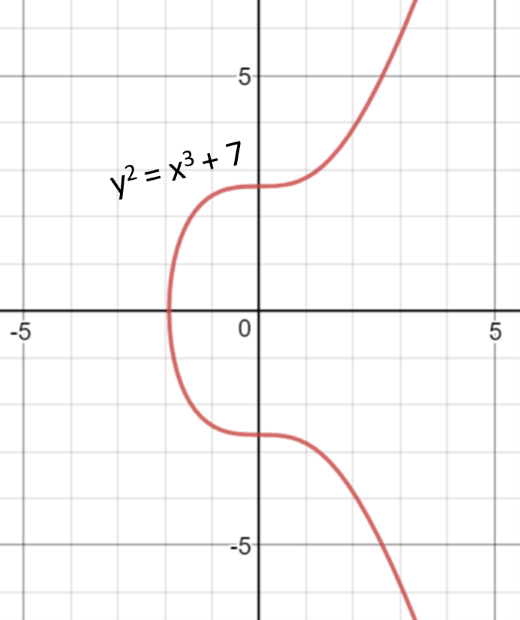
\includegraphics[width=4cm]{img/elliptic-curve.png} 
\end{center}
\caption{Curva ellittica Ethereum $y^{2}=x^{3}+7$}
\end{figure}

\newpage
\subsection{Chiave pubblica}
Una chiave pubblica di Ethereum è un punto su una curva ellittica, il che significa che è un insieme di coordinate x e y che soddisfano l'equazione della curva ellittica.
In termini più semplici, una chiave pubblica di Ethereum è costituita da due numeri, uniti insieme. Questi numeri sono prodotti dalla chiave privata mediante un calcolo che può andare solo in un verso . Ciò significa che è banale calcolare una chiave pubblica se si dispone della chiave privata, ma è computazionalmente difficile calcolare la chiave privata dalla chiave pubblica.\\
La chiave pubblica viene calcolata dalla chiave privata mediante l'operazione di  moltiplicazione sulla curva ellittica, che è praticamente irreversibile: K=k*G , dove k è la chiave privata, G è il punto generatore e K è la chiave pubblica risultante.
La moltiplicazione della curva ellittica non è come la normale moltiplicazione, infatti l'operazione inversa sarebbe trovare il logaritmo discreto, cioè calcolare k se si conosce K.\\

Partendo da una chiave privata sotto forma di un numero generato casualmente k , lo moltiplichiamo per un punto predeterminato sulla curva chiamato punto generatore G per produrre un altro punto sulla curva, che è la corrispondente chiave pubblica K :
K = K * G\\
Il punto generatore è specificato come standard del secp256k1, è lo stesso per tutte le implementazioni di e secp256k1; quindi tutte le chiavi derivate da quella curva usano lo stesso punto G. Poiché il punto generatore è sempre lo stesso per tutti gli utenti di Ethereum, una chiave privata k moltiplicata per G comparirà sempre nella stessa chiave pubblica K . La relazione tra k e K è fissa, ma può essere calcolata solo in una direzione, da k a K . Ecco perché un indirizzo Ethereum (derivato da K ) può essere condiviso con chiunque e non rivela la chiave privata dell'utente k.
La moltiplicazione di k * G equivale all'addizione ripetuta, quindi G + G + … + G , ripetuta k volte. In sintesi, per produrre una chiave pubblica K da una chiave privata k , aggiungiamo il punto generatore G a se stesso, k volte.

\subsection{Algoritmo ECDSA}
Ethereum utilizza l'algoritmo di firma: Elliptic Curve Digital Signature Algorithm (ECDSA). Esso viene utilizzato per creare una firma digitale che consente la verifica da parte di terzi senza compromettere la sicurezza.\\
L'algoritmo ECDSA funziona attraverso un meccanismo di crittografia chiamato crittografia asimmetrica. Questo sistema di firma genera due chiavi denominate chiave privata e chiave pubblica . Entrambi i tasti sono correlati da una complessa operazione matematica eseguita su una funzione di curva ellittica. Tutti argomenti di cui abbiamo già trattato.\\
\subsubsection{Meccanismo di firma}
\begin{figure}[htbp] 
\begin{center}
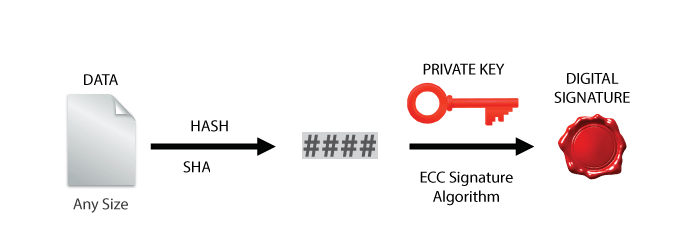
\includegraphics[width=8cm]{img/s.png} 
\end{center}
\caption{Meccanismo di firma ECDSA \cite{SHA}}
\end{figure}
I parametri iniziali sono: l'equazione della curva ellittica usata, \textbf{G} il punto base della curva, cioè un generatore della curva ellittica e \textbf{n} l'ordine intero di \textbf{G} tale per cui $n*G=O$. Ora immaginiamo che ci siano due persone denominate Alice e Bob.  Alice genera una coppia di chiavi, una privata \textbf{$d_{A}$} e una pubblica \textbf{$Q_{A}$}.\\ Per generare una firma per il messaggio \textbf{m}, Alice svolge i seguenti passi:
\begin{enumerate}
\item Calcola e=HASH(m), la quale è una funzione crittografica come SHA-3
\item Sia z la stinga formata dai $L_{n}$ bit più a sinistra di $e$, e dove $L_{n}$ è la lunghezza in bit del gruppo di ordine $n$
\item Si seleziona in modo casualmente sicuro un intero k dell'intervallo $[1,n-1]$
\item Si calcola il punto della curva $(x_{1},y_{1}) = k*G$
\item Si calcola $r=x_{1}$ $mod$ $n$. Se r=0 si ritorna al passo 3.
\item Si calcola $s=k^{-1}(z+rd_{A})$ $mod$ $n$. Nel caso $s=0$ si torna al passo 3.
\item La firma è la coppia $(r,s)$ 
\end{enumerate}

Alcuni dettagli:\\
Attraverso la computazione di s, la stringa z risultante da $HASH(m)$ deve essere convertita ad intero.\\
Come viene stabilito dagli standard, è fondamentale che vengano selezionati k diversi per firme diverse, altrimenti al passo 6 possiamo risolvere l'equazione attraverso $d_{A}$.\\
Date due firme $(r,s)$ e $(r,s')$ impiegare la stessa $k$ per due messaggi $m$ e $m'$ si apre una vulnerabilità ad attacchi.\\
Un aggressore può calcolare $z$ e $z'$ e visto che $s-s'=k^{-1}(z-z')$ l'aggressore può trovare $k=\frac{z-z'}{s-s'}$. Visto che $s=k^{-1}(z+rd_{A})$ l'aggressore può ora calcolare la chiave privata $d_{A}=\frac{sk-z}{r}$.

\subsubsection{Verifica della firma}
\begin{figure}[htbp] 
\begin{center}
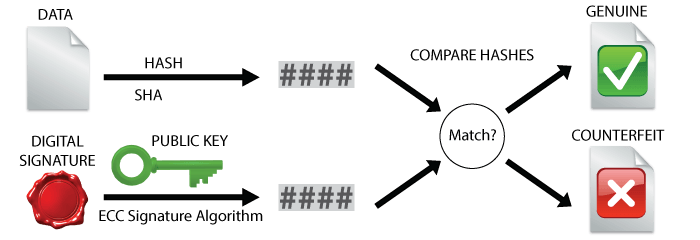
\includegraphics[width=8cm]{img/E.png} 
\end{center}
\caption{Meccanismo di verifica della firma ECDSA. \cite{SHA}}
\end{figure}
Ora Bob deve autenticare la firma di Alice, e questo può farlo solo essendo in possesso della chiave pubblica $Q_{A}$.\\
Come primo passo deve verificare che $Q_{A}$ sia un punto valido della curva:
\begin{enumerate}
\item Controllare che $Q_{A}$ non sia uguale all'elemento neutro. $O$
\item Controllare che $Q_{A}$ appartenga alla curva.
\item Controllare che $n*Q_{A}=O$ 
\end{enumerate}
Dopo aver compiuto questi passi principali Bob:
\begin{enumerate}
\item Verifica che $r$ r $s$ siano interi e compresi tra $[1,n-1]$, in caso contrario la firma non è valida.
\item Esegue la funzione $e=HASH(m)$, con HASH stessa funzione usata durante la generazione.
\item Sia $z$ la stringa formata dai $L_{n}$ bit più a sinistra di $e$.
\item Calcola $w=s^{-1}$ $mod$ $n$
\item Calcola $u_{1} = zw$ mod $n$ e $u_{2} = rw$ mod $n$
\item Calcola il punto della curva $(x_{1},y_{1}) = u_{1}*G+u_{2}*Q_{A}$
\item La firma è valida se $r\equiv x_{1}$ $mod$ $n$, se non è così la firma non è accettata.
\end{enumerate}
\subsubsection{Correttezza dell'algoritmo}
\begin{itemize}
\item Denotiamo con $C$ il punto della curva calcolato al passo 6 della verifica.\\
$C=u_{1}*G+u_{2}*Q_{A}$
\item La chiave pubblica può essere definita anche come $Q_{A}=d_{A}*G$.\\
$C=u_{1}*G+u_{2}*d_{A}*G$
\item Applichiamo la proprietà distributiva.\\
$C=(u_{1}+u_{2}d_{A})*G$
\item Ora espandiamo la definizione di $u_{1}$ e $u_{2}$ dal passo 5 dell'algoritmo di verifica e raccogliamo $s^{-1}$.\\
$C=(z+rd_{A})s^{-1}*G$
\item Ora espandiamo $s$ dal passo 6 dell'algoritmo di generazione della firma.\\
$C=(z+rd_{A})(z+rd_{A})^{-1}(k^{-1})^{-1}*G$
\item Semplificando\\
$C=k*G$
\end{itemize}
Dalla definizione di $r$ questo è il passo 6 dell'algoritmo di verifica.
Quindi possiamo dire che il messaggio firmato supera la verifica.


\chapter{Proof of Work (PoW) vs Proof of Stake (PoS)}
Proof of Work (PoW) e Proof of Stake (PoS) sono gli algoritmi di consenso più famosi per le blockchain.\\
Come abbiamo già citato, gli algoritmi di consenso sono delle procedure che avvengono all'interno di un sistema distribuito e permettono di accordare i nodi sull'esecuzione di regole che definiscono il protocollo della rete. Cioè per validare le transazioni che avvengono sulla rete, oppure per penalizzare quando si verificano delle irregolarità.

\section{Protocolli e meccanismi di consenso}
Molte volte i due termini vengono confusi. Il consenso è una parte software, la quale ha il compito di controllare che le regole vengano rispettate, cioè di convalidare le transazioni, controllare tutte le firme, verificare i saldi di specifici address e controllare che le regole del protocollo siano rispettate. Un esempio sono proprio il PoW e il PoS.


\section{Algoritmo di consenso Proof of Work}
Questo algoritmo corrisponde al Mining, processo che abbiamo già analizzato in precedenza, in cui calcolatori molto potenti cercano di risolvere un problema estremamente complesso al fine di trovare una soluzione e ricevere in cambio una ricompensa per il lavoro svolto.\\
Dopo che ciò si verifica, i miner convalidano un blocco e lo aggiungono alla blockchain, ma prima di farlo devono avere il consenso da parte dei nodi i quali, per concederglielo, devono verificare che l'hash trovato sia corretto.\\
Quindi si ha la necessità di avere computer appositi in grado di risolvere questi problemi, semplicemente perché il primo ad arrivare e a trovare la soluzione riceve la ricompensa. 

\section{Algoritmo di consenso Proof of Stake}
\begin{figure}[htbp] 
\begin{center}
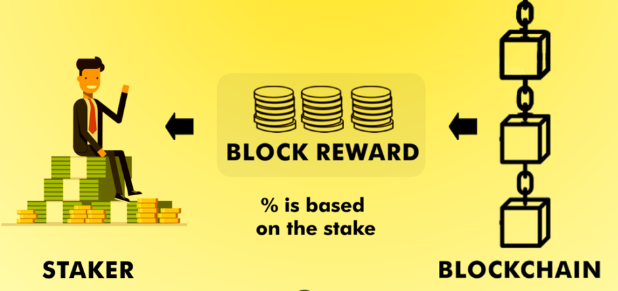
\includegraphics[width=8cm]{img/pos.png} 
\end{center}
\caption{La Proof of Stake. \cite{stake}}
\end{figure}
L'obiettivo dell'algoritmo è sempre convalidare i blocchi, ma la sua procedura avviene in maniera completamente differente. Infatti, esso non è un procedimento fisico, non ci sono dei computer che devono risolvere calcoli complessi ma esistono dei \textbf{validator}.
Un algoritmo di consenso Proof of Stake può essere definito come un insieme di regole che gestiscono una rete blockchain e la creazione della sua moneta; ha quindi anche lui lo stesso obiettivo di un algoritmo Proof of Work, cioè è anch'esso una procedura per raggiungere il consenso. 
Al posto dei miner, i partecipanti alla rete che vogliono far parte della convalida delle transazioni e quindi nella creazione di blocchi, devono detenere una certa quota di valuta nella rete, per esempio attraverso un portafoglio collegato alla sua blockchain. Questo processo è noto come staking, cioè una parte di fondi vengono bloccati per un certo periodo ed usati per convalidare blocchi. Tuttavia, un creatore di blocchi in un sistema PoS può solo creare blocchi proporzionati alla propria partecipazione in stake alla rete.
Le reti PoS sono basate su algoritmi deterministici, quindi i validatori dei blocchi sono scelti in base alla quantità di valuta che hanno messo in stake. Tuttavia, il saldo non deve essere il solo parametro da guardare, perché potrebbe potenzialmente portare a una centralizzazione, infatti i membri ricchi di una rete godrebbero di grandi vantaggi; quindi ogni blockchain aggiunge dei parametri affinché ci sia omogeneità.

\subsection{Dettagli approfonditi del Proof of stake}
Per iniziare, supponiamo di avere un insieme di N validatori V = {V1,...,VN} e che ogni validatore V appartenenete a  V abbia una quantità di puntata W(V), un numero reale positivo che descrive una quantità di garanzie. Facciamo l'ulteriore ipotesi che l'importo medio della puntata per ogni validatore sia 1 unità, quindi la somma della puntata totale è N. Tutte le nostre operazioni che coinvolgono lo stake saranno lineari, quindi questo ridimensionamento non cambia la situazione e rende più facile la contabilità. Supponiamo che i set di validatori e le dimensioni delle puntate siano fissi per concentrarci sugli elementi teorici essenziali del protocollo.\\
Gli elementi principali del protocollo sono:

\begin{itemize}
\item Funzione di scelta della fork(): che, quando viene data una vista G, identifica un singolo blocco foglia B. Questa scelta produce una catena unica fork(G) = chain(B) dalla $B_{genesi}$  alla B-esima chiamata alla catena canonica. Il blocco B è chiamato la testa della catena nella vista  di G. Intuitivamente, una regola di scelta del fork dà a un validatore una legge da seguire per decidere quale dovrebbe essere il blocco "giusto". Ad esempio, la regola della catena più lunga è una regola di scelta del fork che restituisce il blocco foglia che è più lontano dal blocco di genesi
\item Concetto di finalità: cioè una funzione deterministica F, data una vista G, restituisce un insieme F(G) di  blocchi finalizzati. Intuitivamente, i blocchi finalizzati sono blocchi che fanno parte della storia della blockchain.
\item Condizioni di taglio: queste sono condizioni che i validatori onesti non violerebbero mai e i validatori che non le rispettino possono essere scoperti in modo dimostrabile con l'idea che la posta in gioco (stake) dei trasgressori sarebbe stata diminuita o distrutta. Le condizioni di taglio incentivano i validatori a seguire il protocollo, ed è proprio lui che può premiare i validatori onesti per aver catturato validatori disonesti che violano le condizioni.
\end{itemize}

Il concetto chiave che usiamo per definire questi elementi principali sono le attestazioni, le quali sono voti (incorporati nei messaggi) che decidono quali blocchi dovrebbero essere a capo della catena. Per impedire ai validatori di votare due volte o votare in modi che violano il protocollo, applichiamo condizioni di taglio che possono essere utilizzate per distruggere la partecipazione di un validatore, incentivando i validatori a seguire le regole.

\begin{figure}[htbp] 
\begin{center}
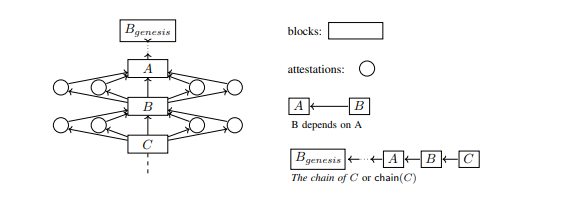
\includegraphics[width=8cm]{img/imgPoS.png} 
\end{center}
\caption{Vista ideale con blocchi e attestazioni.}
\end{figure}

Si può vedere una versione idealizzata del protocollo in figura, in ogni periodo di tempo, viene creato un nuovo blocco attraverso il blocco padre che è proprio l'ultima testa della catena (che è idealmente solo l'ultimo blocco creato) e i validatori nel comitato corrispondente attestano perfettamente il nuovo blocco. In situazioni meno idealizzate, i blocchi possono biforcarsi oppure potremmo avere attestazioni mancanti e le attestazioni entreranno in gioco aiutando i validatori a decidere la testa corretta della catena.

\section{Caratteristiche degli algoritmi di consenso}
Quindi le caratteristiche di un algoritmo di consenso devono essere principalmente due:
\begin{itemize}
\item sicurezza: l'insieme dei blocchi finalizzati F(G) per qualsiasi vista G non può mai contenere due blocchi in conflitto.
\item liveness: l'insieme dei blocchi finalizzati può effettivamente crescere. Ci sono diversi modi per definire la liveness. Il protocollo deve averne almeno due:
\begin{itemize}
\item liveness plausibile: se indipendentemente da eventuali eventi precedenti come attacchi da persone malevoli o latenza è sempre possibile finalizzare nuovi blocchi ed è impossibile andare in deadlocked. Questo per prevenire situazioni in cui i validatori onesti non possano continuare.
\item. liveness probabilistica: se indipendentemente da eventuali eventi precedenti, è probabile che nuovi blocchi vengano finalizzati (una volta fatte alcune ipotesi probabilistiche sulla latenza della rete e sulle capacità degli aggressori).
\end{itemize}
\end{itemize}

\section{Ethereum}
Dalla sua creazione Ethereum è passato dall'algoritmo di consenso Proof of work al Proof of stake. Questo per diversi motivi che affronteremo in seguito, ma prima descriviamo queste due procedure nel dettaglio per Ethereum.

\subsection{Ethereum PoW}
Come abbiamo citato in precedenza il processo PoW si basa sul mining, in particolare l'algoritmo di mining di ethereum è denominato Ethash ed è considerato uno degli algoritmi più elaborati nel mondo delle criptovalute. Esso è un algoritmo che utilizza tecniche informatiche elaborate per garantire la massima sicurezza possibile.\\
L'algoritmo Ethash si basa su due principi chiave:
\begin{enumerate}
\item E' resistente al mining ASIC (cioè a minatori con potentissime tecnologie)
\item Efficiente e facilmente verificabile da tutti i client.
\end{enumerate}

\subsubsection{Funzionamento di Ethash}
Possiamo definire formalemnte Ethash in questo modo:\\
\begin{center}
$ (m,n) = PoW(\textit{H}_{m},\textit{H}_{n},d) $
\end{center}
Dove m è mixHash, n è il nonce, $H_{m}$ è l'intestazione del nuovo blocco con esclusi nonce e mixHash che devono essere calcolati, $H_{n}$ è il nonce dell'intestatario del blocco e d è il DAG (set di dati di grandi dimensioni).\\
Ora descriviamo le basi del funzionamento di Ethash:
\begin{itemize}
\item Un seme calcolato viene creato attraverso le intestazioni di blocco fino a quando inizierà la procedura di mining.
\item  Questo seme viene utilizzato per il calcolo e la generazione di una cache pseudo-casuale da 16 MB.
\item Questa cache è utilizzata per la generazione di un insieme di dati molto più grande di 4GB, il DAG. Esso è semipermanente e viene aggiornato circa ogni 30mila blocchi. In questo modo il DAG varia.
\item Una volta generato il DAG, può iniziare il mining. Questo processo combina i valori casuali provenienti dal DAG con i dati forniti dalla rete e le transazioni da verificare.
\item Infine la verifica viene eseguita attraverso un processo che rigenera parti specifiche dell'insieme di dati utilizzando la memoria cache, in modo tale da velocizzare questo processo.\\
\end{itemize}
Le funzioni Keccak-256 e Keccak-512 sono usate durante il processo, un algoritmo da cui è stato derivato lo standard SHA-3.\\
Esiste il vincolo che rende tale algoritmo strettamente legato alla memoria ed in particolare al bandwidth, cioè al bus, che consiste proprio nella velocità di accesso al DAG per il fetch dei dati.
Durante il processo avvengono così tante revisioni e modifiche perchè queste operazioni rispondono alla risoluzione di problemi, ottimizzazioni, vulnerabilità e modifiche per rendere il lavoro più complesso per gli ASIC e più semplici per le GPU.\\

\subsubsection{Keccak-256}
Il meccanismo di hash crittografico Keccak-256 è un algoritmo di hash crittografico che viene utilizzato da Ethereum per proteggere i dati sensibili, come le chiavi private degli utenti. In pratica, l'algoritmo Keccak-256 converte un input di dati di lunghezza variabile in una stringa di lunghezza fissa di 256 bit, chiamata hash. Questa operazione di hash è irreversibile, il che significa che non è possibile recuperare l'input originale dai dati di output.\\
L'algoritmo Keccak-256 utilizza una funzione di compressione iterativa per elaborare i dati di input. Essa si basa su una serie di operazioni matematiche, tra cui XOR, permutazioni e sostituzioni. In particolare, l'algoritmo Keccak-256 utilizza una funzione di permutazione chiamata "Rho" che ruota i bit all'interno di uno stato interno dell'algoritmo. Questa rotazione dei bit è il cuore della sicurezza dell'algoritmo e rende l'hash resultante molto resistente ai tentativi di hacking.\\
La funzione rho è composta da una serie di rotazioni cicliche di bit che sono definite da un insieme di costanti predefinite. Le roatazioni sono definite come segue: per ogni valore di x e y (dove x e y sono interi), la funzione rho esegue una rotazione ciclica di y bit in direzione destra su un bit specifico all'interno dello stato interno dell'algoritmo. Il bit specifico è calcolato utilizzando la seguente formula:
\begin{center}
    $i = ((y + 2) * x + y)$ $mod$ $w$
\end{center}
dove w è la larghezza del registro interno dell'algoritmo (1600 bit per Keccak-256).
Una volta che l'indice i è stato calcolato, la funzione rho ruota il bit all'indice i di y posizioni in direzione destra. Questo processo viene ripetuto per una serie di costanti predefinite, che determinano l'ordine delle rotazioni cicliche e il numero di bit di rotazione.\\
Per generare l'hash Keccak-256 di un determinato input di dati, l'algoritmo esegue i seguenti passaggi:
\begin{enumerate}
    \item \textbf{Preparazione dei dati di input}: viene convertito l'input di dati in una serie di blocchi di 1088 bit, dove ogni blocco contiene il messaggio di input e un valore di padding.
    \item \textbf{Assorbimento dei dati}: l'algoritmo assorbe i blocchi di dati di input in uno stato interno, utilizzando la funzione di compressione iterativa.
    \item \textbf{Finale}: una volta che tutti i blocchi di dati di input sono stati assorbiti, l'algoritmo genera l'hash finale utilizzando la funzione di compressione e applicando alcuni passaggi di output per generare una stringa di 256 bit.
\end{enumerate}
In generale, l'algoritmo Keccak-256 è considerato sicuro poiché è resistente ai tentativi di hacking noti, come la collisione degli hash (cioè la creazione di due input diversi che producono lo stesso hash di output). Inoltre, l'algoritmo è stato selezionato per la sua resistenza alle attività di crittoanalisi e alle vulnerabilità di tipo backdoor.

\subsubsection{Keccak-256 preudocodice}
Per approfondire maggiormente questo algoritmo di hashing viene fornito lo pseudocodice e spiegato nel modo più dettagliato possibile, esso è stato integrato dalla documentazione ufficiale di Ethereum \cite{ETH}:
\begin{algorithm}
\caption{Algoritmo di hash crittografico Keccak-256}
\begin{algorithmic}[1]
\State Definizione delle costanti dell'algoritmo:
\State $\quad$ const $r = 1600$, $c = 512$, $b = 1600 - c$
\State Definizione delle costanti per la funzione di permutazione Rho:
\State $\quad$ const RC = [0x0000000000000001, 0x0000000000008082, ...]
\State Funzione di compressione:
\Function{Keccak-256}{message: byte array} $\rightarrow$ {hash: byte array}
\State Inizializzazione dello stato interno dell'algoritmo:
\State $\quad$ var state[r/c][c] := 0
\State $\quad$ var block := pad(message)
\State Assorbimento dei blocchi di dati di input:
\For{each $b$ in $block$}
\State $\quad$ state := state $\oplus$ $b$
\State $\quad$ state := KeccakF(state)
\EndFor
\State Generazione dell'hash di output:
\State $\quad$ var hash := ""
\For{each $row$ in $state$}
\For{each $lane$ in $row$}
\State $\quad$ hash := hash || $lane$
\EndFor
\EndFor
\State \Return $hash$
\EndFunction
\State Funzione di padding:
\Function{pad}{message: byte array} $\rightarrow$ {block: byte array}
\State $\quad$ var block := []
\State $\quad$ var padLen := (-len(message) - 2 * b) mod b
\State $\quad$ var pad := [0x01] + [0x00] * (padLen - 1) + [0x80]
\State $\quad$ block := message || pad
\State \Return $block$
\EndFunction

\State Funzione di permutazione:
\Function{KeccakF}{state: array} $\rightarrow$ {array}
\For{i := 0 to 23}
\State $\quad$ C := [state[x, y] $\oplus$ RC[i] for x := 0 to 4]
\State $\quad$ D := [C[(x-1) mod 5] $\oplus$ rot(C[(x+1) mod 5], 1) for x := 0 to 4]
\State $\quad$ state := state $\oplus$ D
\State $\quad$ state := Rho(state)
\State $\quad$ state := Pi(state)
\State $\quad$ state := Chi(state)
\State $\quad$ state[0, 0] := state[0, 0] $\oplus$ RC[i]
\EndFor
\State \Return $state$
\EndFunction
    \algstore{myalg}
\end{algorithmic}
\end{algorithm}

\begin{algorithm}
\begin{algorithmic}[1]
    \algrestore{myalg}
\State Funzione di rotazione:
\Function{rot}{a: bit string, n: int} $\rightarrow$ {bit string}
\State $\quad$ \Return $(a \gg (n \bmod w)) \lor (a \ll (w - (n \bmod w)))$
\EndFunction

\State Funzione di permutazione Rho:
\Function{Rho}{state: array} $\rightarrow$ {array}
\State $\quad$ var A := state
\For{j := 0 to 23}
\State $\quad$ var x := 1, y := 0, t := A[x, y]
\For(i := 0 to 23)
\State $\quad\quad$ var newX := y, newY := (2x + 3y) mod 5
\State $\quad\quad$ t, A[newX, newY] := A[newX, newY], rot(t, (i+1)(i+2)/2)
\State $\quad\quad$ x, y := newX, newY
\EndFor
\EndFor
\State \Return $A$
\EndFunction
\State Funzione di permutazione Pi:
\Function{Pi}{state: array} $\rightarrow$ {array}
\State $\quad$ var A := state
\State $\quad$ var B := A
\For{x := 0 to 4}
\For(y := 0 to 4)
\State $\quad\quad$ newX := (3x + 2*y) mod 5
\State $\quad\quad$ newY := (x + y) mod 5
\State $\quad\quad$ B[x, y] := A[newX, newY]
\EndFor
\EndFor
\State \Return $B$
\EndFunction
\State Funzione di permutazione Chi:
\Function{Chi}{state: array} $\rightarrow$ {array}
\State $\quad$ var A := state
\State $\quad$ var B := A
\For(y := 0 to 4)
    \State $\quad\quad$ B[x, y] := C[x]
\EndFor
\State \Return $B$
\EndFunction
\end{algorithmic}
\end{algorithm}

\newpage
Come si può vedere dallo pseudocodice, l'algoritmo Keccak-256 si basa sulla funzione di permutazione KeccakF che viene eseguita su una matrice di stato di 5x5 byte. Questa funzione esegue 24 round di permutazioni su questa matrice, dove ogni round utilizza una costante RC specifica, che viene combinata con gli elementi della matrice di stato attraverso operazioni XOR. In ogni round, la matrice di stato viene anche sottoposta a tre funzioni di permutazione Rho, Pi e Chi, che combinano la posizione degli elementi della matrice di stato in modi specifici.

L'algoritmo Keccak-256 è un esempio di funzione hash crittografica a flusso di cifratura, il che significa che la sua uscita viene generata in modo continuo e dipende solo dall'input corrente. L'algoritmo utilizza una serie di operazioni di permutazione e rotazione per diffondere l'input su tutta la matrice di stato, rendendolo difficile per un attaccante invertire l'operazione e determinare l'input originale. Questa proprietà di sicurezza è fondamentale per garantire la sicurezza delle transazioni sulla blockchain.\\
Ora analizziamo lo pseudocodice:
\begin{enumerate}
    \item \textbf{Definizione delle costanti dell'algoritmo}: la larghezza del percorso di dati r, la larghezza della capacità c e la larghezza del percorso del bit di stato b (1600 - c).
    \item \textbf{Definizione delle costanti per la funzione di permutazione Rho}: utilizzo di una serie di costanti chiamate RC, che vengono utilizzate all'interno della funzione di permutazione Rho. Ci sono 24 costanti RC, ognuna delle quali è una costante di 64 bit.
    \item \textbf{Funzione di compressione}: La funzione di compressione è il nucleo dell'algoritmo. Accetta un blocco di dati di input e restituisce un blocco di output compresso. Essa inizia inizializzando lo stato interno dell'algoritmo a zero. Il blocco di dati di input viene quindi assorbito nel percorso del bit di stato attraverso l'operazione XOR. Dopo aver assorbito un blocco di dati di input, la funzione Rho viene applicata allo stato interno dell'algoritmo.
    \item \textbf{Generazione dell'hash di output}: Dopo aver assorbito tutti i blocchi di dati di input e aver applicato la funzione di permutazione Rho, viene generato un hash di output. Il percorso del bit di stato viene concatenato in un unico flusso di bit, che costituisce l'hash di output finale.
    \item \textbf{Funzione di padding}: Prima di assorbire i dati di input, la funzione di padding viene applicata ai dati di input. Il padding consiste in un bit di inizio, seguito da un numero variabile di bit nulli e un bit finale di 1. La lunghezza totale dei dati di input, compreso il padding, deve essere un multiplo di 512 bit.
    \item \textbf{Divisione in blocchi}: Dopo aver applicato la funzione di padding, i dati di input vengono divisi in blocchi di 512 bit ciascuno. Se l'ultimo blocco non è completo (cioè non contiene 512 bit), viene ulteriormente riempito con bit nulli.
    \item \textbf{Inizializzazione dello stato interno}: L'algoritmo Keccak-256 utilizza uno stato interno che viene inizializzato a zero.
    \item \textbf{Assorbimento dei dati di input}: I blocchi di dati di input vengono assorbiti nel percorso del bit di stato tramite l'operazione XOR.
    \item \textbf{Applicazione della funzione di permutazione Rho}: Dopo aver assorbito un blocco di dati di input, la funzione di permutazione Rho viene applicata allo stato interno dell'algoritmo. La funzione Rho utilizza le costanti RC per effettuare una serie di operazioni di rotazione su un insieme di posizioni all'interno dello stato interno.
    \item \textbf{Generazione dell'hash di output}: Dopo aver assorbito tutti i blocchi di dati di input e aver applicato la funzione di permutazione Rho, viene generato un hash di output. Il percorso del bit di stato viene concatenato in un unico flusso di bit, che costituisce l'hash di output finale.
    \item \textbf{Restituzione dell'hash di output}: L'hash di output viene restituito come risultato dell'algoritmo.
\end{enumerate}
\subsubsection{Funzionamento approfondito di Ethash}
\begin{figure}[htbp] 
\begin{center}
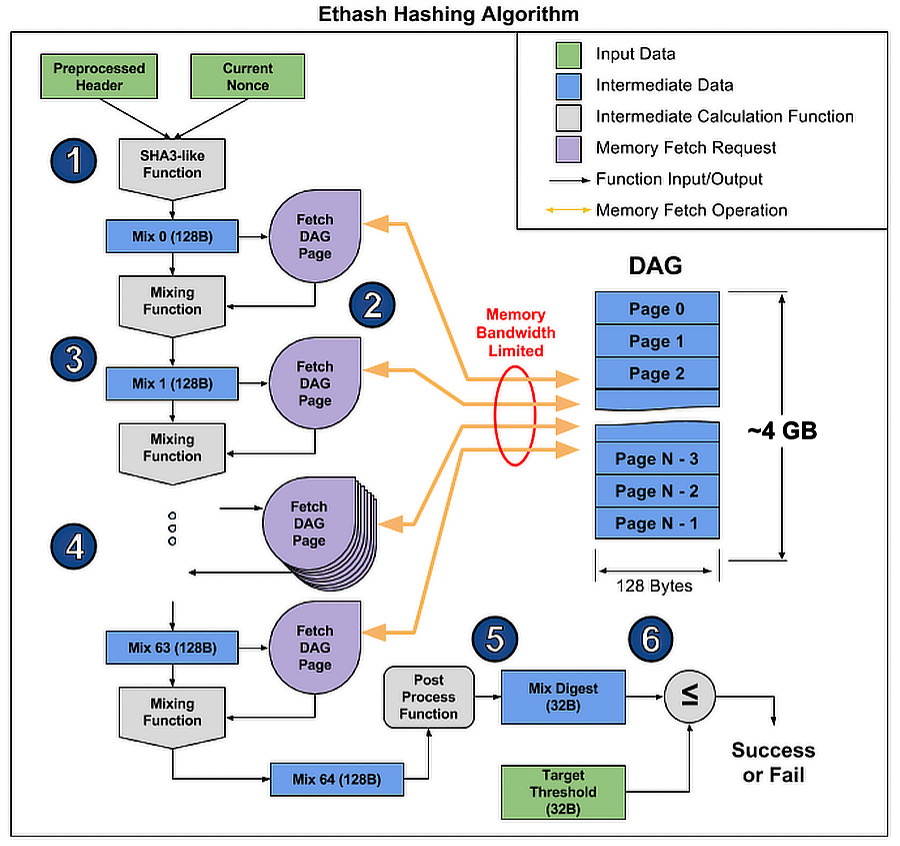
\includegraphics[width=8cm]{img/ethash.jpg}
\end{center}
\caption{Ethash hashing algorithm. \cite{etlash}}
\end{figure}
\begin{enumerate}
\item Come primo passo vengono combinati insieme attraverso lo SHA-3 un header preprocessato proveniente dall'ultimo blocco ed il Nonce attuale, cioè un numero casuale di 32 bit generato dai minatori come target del hash. Quindi viene creata una sequenza di Byte lunga 128, chiamata Mix 0.
\item Il Mix 0 viene usato per determinare quali dati collezionare dalla DAG, attraverso una funzione di fetch.
\item Il Mix 0 ed i dati recuperati dal DAG vengono mescolati, creando una stringa di 128 Byte, chiamata Mix 1.
\item  L'operazione 3 viene ripetuta con lo stesso procedimento per 64 volte, fino ad ottenere il Mix 64.
\item Il Mix 64 viene processato affinché si ottenga una sequenza di 32 Byte, denominata Mix Digest.
\item La sequenza viene confrontata con una seconda sequenza target. Se la prima risulta minore del target, allora possiamo considerare il Nonce come raggiunto e inizia il processo di broadcasting sulla rete Ethereum. In caso contrario, l'algoritmo viene di nuovo eseguito con un nuovo Nonce.
\end{enumerate}

\subsubsection{Caratteristiche dell'algoritmo Ethash}
\begin{itemize}
\item L'algoritmo dipende fortemente dalle operazioni, le quali usano un grande quantitativo di RAM, consumando grandi quantitativi di banda.
\item L'algoritmo è compatibile con le operazioni svolte dalla GPU, esso infatti usa la memoria della GPU per tenere l'intero DAG in memoria e anche grazie all'utilizzo della cache permette di eseguire tutti i calcoli dell'area di lavoro a grande velocità.
\item Offre anche eccellenti capacità di verifica da parte dei client più piccoli, infatti con appena 16 MB di RAM, è possibile verificare le transazioni in modo veloce.
\end{itemize}

\subsubsection{Vantaggi e svantaggi dell'algoritmo}
\textbf{VANTAGGI}\\
\begin{itemize}
\item Algoritmo di semplice implementazione, sicuro e pratico. In aggiunta è anche resistente agli ASIC.
\item E' estremamente veloce, con l'uso del DAG in memoria e della cache che lo rendono efficiente nella produzione di blocchi. Questo permette di avere un tempo di convalida adattabile cercando sempre l'equilibrio tra sicurezza e scalabilità.
\end{itemize}
\textbf{SVANTAGGI}\\
\begin{itemize}
\item Il sistema per calcoli veloci richiede un ampio uso di memoria e potrebbe essere un problema per computer più modesti.
\item Esistono macchinari in grado di minare estremamente facilmente ethereum e questo ha iniziato a portare a una centralizzazione del mining su Ethereum, proprio per questo è stato introdotto Ethereum 2.0 il quale prevede l'abbandono del Proof of Work e con lui anche Ethash come algoritmo di mining, in cambio di un Proof of Stake.  
\end{itemize}

\subsection{Ethereum PoS}
Nell'algoritmo di proof-of-stake, i validatori mettono in gioco del capitale attraverso il processo di staking sotto forma di ether in uno smart contract su Ethereum. Questa moneta, denominata ether in staking gioca da garanzia, cioè essa può essere distribuita se il validatore si comporta in modo disonesto o pigro. Il validatore ha la responsabilità di verificare che i nuovi blocchi propagati in rete siano validi, ma ha anche la possibilità di creare e propagare nuovi blocchi. \\
Questo protocollo permette anche di evitare quasi del tutto gli attacchi di tipo 51\%. I quali verranno trattati nella prossima sezione.

\subsubsection{I validatori}
Per diventare un validatore, un utente deve depositare 32 ETH nel contratto di deposito e eseguire tre software distinti: un client d'esecuzione, uno di consenso e anche uno di validatore.\\
Una volta depositati gli ether, l'utente si mette in una coda, in attesa di essere attivati. Una volta attivi, gli utenti iniziano a ricevere blocchi dai peer della rete. Le transazioni presenti nel blocco appena arrivato vengono eseguite nuovamente e la firma del blocco viene verificata, per accertarsi che il blocco sia valido. A questo punto il validatore invia nella rete un voto, il quale è chiamato \textbf{attestazione}.\\

A differenza del PoW la difficoltà di esecuzione di questa operazione è fissa. In aggiunta, il tempo di Ethereum di PoS è diviso in \textbf{slot} da 12 secondi ed in \textbf{epoche}, le quali sono formate da 32 slot. In ogni slot viene selezionato un validatore in modo casuale come propositore di blocchi. Esso è responsabile della creazione di un nuovo blocco e dell'invio di esso ad altri nodi sulla rete. In aggiunta, in ogni slot è scelto un comitato di validatori, i cui voti determinano la validità del nuovo blocco. 

\subsubsection{Finalità}
Possiamo dire che una transazione ha una finalità quando fa parte di un blocco, il quale non può cambiare senza bruciare un quantitativo di ether, Ethereum lo gestisce usando i blocchi definiti checkpoint. In ogni epoca il primo blocco è un checkpoint. I validatori votano per le coppie di checkpoint che considerano valide. Se una coppia di checkpoint riceve almeno i due terzi di voti dell'ether in staking totale, i checkpoint  si aggiornano. Ora il blocco è aggiornato e finalizzato.\\
Giunti a questo punto il ripristino di un blocco finalizzato da parte di una persona malevola ha un costo di almeno un terzo della domanda totale di ether in staking.\\
Poiché il completamento richiede una maggioranza dei due terzi, un utente potrebbe impedire alla rete di raggiungere il completamento votando con un terzo dello stake totale. Ma questo non è possibile visto che esiste un meccanismo per difendersi da questa eventualità ed è chiamata \textbf{perdita per inattività}. Essa si attiva ogni volta che la catena non raggiunge il completamento per più di quattro epoche. Il meccanismo disperde l'ether ricevuto in staking dai validatori che hanno votato la maggioranza, in modo tale da consentire di ottenere nuovamente una maggioranza di due terzi e di finalizzare la catena.

\subsubsection{Sicurezza cripto economica}
La gestione di un validatore è un impegno molto grande. Il validatore deve avere connettività e hardware sufficienti per partecipare alla validazione dei blocchi. Come ricompensa  riceve in cambio degli ether, i quali si aggiungono al suo saldo in staking. Tuttavia, alcuni utenti potrebbero cercare un modo per ricavare del profitto personale o cercare di sabotare il meccanismo. Affinché non avvenga, i validatori se non partecipano quando richiesto perdono la ricompensa e il loro stake esistente può essere distrutto se il loro comportamento è disonesto. I comportamenti considerabili disonesti sono: 
\begin{itemize}
\item Proporre diversi blocchi in uno slot singolo (equivoco).
\item Invio di attestazioni contraddittorie. 
\end{itemize}
L'importo di ether sotratto dallo staking per aver compiuto queste procedure dipende da quanti validatori sono tagliati più o meno in contemporanea. L'azione di sottrarre ether è denominata \textbf{slashing}. Questa è anche nota come \textbf{sanzione di correlazione} e può essere minima oppure può anche comportare la sottrazione di tutto lo stake del validatore. Più il validatore non collabora più sarà sanzionato infatti esistono la sanzione al Giorno 1, la sanzione di correlazione al Giorno 18 e al giorno 36 avviene l'espulsione dalla rete. Ma ogni giorno ricevono altre modeste sanzioni perché sono presenti nella rete ma non inviano voti. Tutto questo porta a un attacco molto costoso per un utente malevolo.

\newpage
\subsubsection{Scelta della biforcazione}
Se la rete opera in modo ottimale, esiste sempre un solo nuovo blocco in testa alla catena e tutti i validatori attestano quel blocco. Tuttavia, è possibile che i validatori vedano in testa alla catena blocchi diversi, a causa della latenza della rete o perché un propositore di blocchi ha equivocato. I client di consenso hanno bisogno di un algoritmo per decidere quale sarà la testa della catena. L'algoritmo usato in Ethereum nel PoS è detto LMD-GHOST e funziona identificando la biforcazione avente il peso di attestazioni più grande nella sua storia.
\begin{figure}[htbp] 
\begin{center}
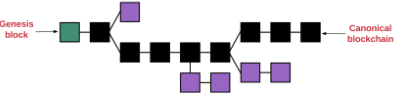
\includegraphics[width=10cm]{img/ghs.png}
\end{center}
\caption{Scelta della fork attraverso la regola di GHOST. \cite{genesis}}
\end{figure}

\subsubsection{Algoritmo LMD GHOST Fork-CHoise rule}
La regola Greediest Heaviest Observed SubTree (GHOST) è una regola di scelta della fork introdotta da Sompolinsky e Zohar.\\ GHOST è un algoritmo avido che fa crescere la blockchain su sotto-rami per la maggior parte della sua attività.\\ Nella ricerca di un protocollo di consenso corretto, Zamfir, un altro ricercatore, introduce un adattamento naturale di GHOST, chiamiamo questa variante: Latest Message Driven Greediest Heaviest Observed SubTree (LMD GHOST), che possiamo definire solo dopo aver avuto una definizione di peso:
data una vista G, sia M l'insieme delle ultime attestazioni, una per validatore. Il peso w(G,B,M) è definito come la somma della quota dei validatori \textit{i} la cui ultima attestazione in M è a B o ai discendenti di B.
L'algoritmo può essere rappresentato in pseudo-codice:\\

\begin{algorithm}
\caption{LMD GHOST (Scelta della Fork)}
\begin{algorithmic}[1]
\Procedure{LMD-GHOST}{$G$}
\State $B \gets B_{Origine} $
\State $M \gets $ la più recente attestazione dei validatori (una per validatore)
\While{B non è una foglia del blocco G}
\State $B \gets $ l'arg massimo $w(G,B',M)$ dove (\textit{B'} è il figlio di \textit{B})
\State (i collegamenti vengono interrotti dall'hash del blocco di header)
\EndWhile \\
\Return{$B$}
\EndProcedure
\end{algorithmic} 
\end{algorithm}

\newpage
L'idea di LMD GHOST è che in qualsiasi fork, vengano usati i pesi dei sottoalberi creati dalla fork e assumiamo che il sottoalbero con il peso più grande sia quello da considerare. 
Con questo algoritmo finiremo sempre a un blocco foglia, che definisce una catena canonica.\\
Un esempio di questo algoritmo può essere questo:\\
\begin{figure}[htbp] 
\begin{center}
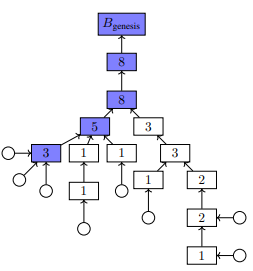
\includegraphics[width=7cm]{img/esGHOST.png}
\end{center}
\caption{Un esempio della regola di scelta del fork LMD-GHOST.}
\end{figure}
\\Il numero in ogni blocco B è il peso, con tutte le attestazioni/convalide (i cerchi) che hanno peso 1 nel nostro esempio. Un validatore che utilizza questa vista concluderà che la catena blu è la catena canonica e produrrà l'ultimo blocco blu a sinistra, con peso 3, per essere la testa della catena.
\newpage
\subsubsection{Vantaggi e Svantaggi dell'algoritmo}
\textbf{VANTAGGI}\\
\begin{itemize}
\item Lo staking rende molto più semplice alle persone di partecipare alla protezione della rete, promuovendo e garantendo la decentralizzazione. Il nodo del validatore può essere eseguito da chiunque e da qualunque computer.\\ Le staking pool prevedono l’unione di più parti per partecipare allo staking come un singolo validatore, in questo modo gli utenti possono convalidare senza avere singolarmente 32 ETH.
\item Non c'è bisogno di potentissimo hardware per il mining.
\item Il PoS garantisce molta più sicurezza del PoW.
\item Permette di risparmiare tantissimo sull'energia consumata, rendendo il progetto maggiormente green.
\end{itemize}
\textbf{SVANTAGGI}
\begin{itemize}
\item E' meno testato del PoW.
\item Il PoS è molto più complesso e gli utenti devono far funzionare tre parti di software per poter partecipare.
\end{itemize}


\subsection{Attacco del 51\%}
Distinguiamo l'attacco nel caso avvenga su una blockchain dove è presente l'algoritmo PoW o PoS.\\
L'attacco del 51\% su una blockchian dove è presente l'algoritmo di consenso Proof-of-work consiste in un gruppo di minatori che controllano oltre il 50\% dell'hash rate di mining (potenza di calcolo) della rete. Possedere questa quantità di potenza di calcolo dei nodi della rete dà alle parti il potere di alterare la blockchain.
Gli aggressori sarebbero in grado di impedire che nuove transazioni ottengano conferme, consentendo loro di sospendere i pagamenti tra alcuni o tutti gli utenti. Sarebbero anche in grado di annullare le transazioni. L'annullamento delle transazioni potrebbe consentire loro di raddoppiare la spesa. \\

Invece, l'attacco del 51\% su una blockchian dove è presente l'algoritmo di consenso Proof-of-stake consiste in un utente malevolo il quale avrebbe il 51\% di ETH in staking, quindi circa \$15.000.000.000 di dollari. In questo modo potrebbe poi usare le proprie attestazioni per garantire che la propria biforcazione, creata appositamente, sia quella con le maggiori attestazioni accumulate. Ed è proprio il peso delle attestazioni accumulate che i client di consenso usano per determinare la catena corretta, in questo modo l'utente potrebbe rendere canonica la propria biforcazione.\\ 
Ma il punto di forza del PoS rispetto al PoW è che gli altri convalidatori potrebbero preparare un contrattacco. Ad esempio, i validatori onesti potrebbero decidere di continuare a validare sulla catena di minoranza e ignorare la biforcazione malevola, incoraggiando app e scambi a fare lo stesso. Potrebbero anche rimuovere l'utente malevolo dalla rete e distruggerne l'ether in staking. \\

Un attacco del 51\% è estremamente difficile e impegnativo su una criptovaluta con un alto tasso di partecipazione. Nella maggior parte dei casi, il gruppo di aggressori dovrebbe poter controllare il 51\% della potenza di calcolo o dello staking e il costo di questa operazione è uno dei fattori più significativi che impediscono questo attacco.

\chapter{Conclusioni}
\section{Conclusioni finali}
In questa relazione ho cercato di approfondire in modo graduale, partendo da definizioni base fino ad arrivare ad aspetti molto profondi sulla struttura delle criptovalute, dei problemi legati ad esse e ciò che le circonda. Ho scelto questo argomento di criptografia, perchè durante le lezioni è quello che mi ha incuriosito di più e nonostante fosse un mondo completamente nuovo per me, credo ora di avere almeno le idee base su questi aspetti. In aggiunta mi ha anche incuriosito il fatto di poter iniziare a sviluppare e creare nuove applicazioni basate sulla rete Ethereum e questo è possibile direttamente online nella pagine principale del sito. Sarebbe bello avere un corso interamente dedicato a questo argomento nel piano di studi, visto quante possibilità offre.   

\begin{thebibliography}{100}
\bibitem{genesis} preethikasireddy.com, Come funziona Ethereum, www.preethikasireddy.com/post. 2017.
\bibitem{smartContract} Salah, Khaled. (2018). IOT Access control and Authentication Management via blockchain. 
\bibitem{albero} theledger.it, Merkle Tree, Theledger Team, 2020.
\bibitem{ether} https://ethereum.org/it/developers/docs, Corwin Smith, 2022
\bibitem{mine} www.javatpoint.com/how-block-hashes-work-in-blockchain, 2020
\bibitem{block} Weber, Ingo \& Lu, Qinghua \& Tran, An Binh \& Deshmukh, Amit \& Gorski, Marek \& Strazds, Markus. (2019). A Platform Architecture for Multi-Tenant Blockchain-Based Systems. 10.1109/ICSA.2019.00019. 
\bibitem{SHA} segger.com, emSecure, 2019
\bibitem{stake} getbtcz.com, 2019
\bibitem{etlash} academy.bit2me.com, José Maldonado, 15 luglio, 2020.
\bibitem{ETH} Ethereum Yellow Paper: Wood, G. (2014). Ethereum: A secure decentralised generalised transaction ledger. Ethereum Foundation. Retrieved from https://ethereum.github.io/yellowpaper/paper.pdf
\end{thebibliography}
\end{document}
